% Figure 2: background-suppression timing, (a) full preparation, (b) zoom on Inv1-Inv2-readout.
% Build (from latex/): pdflatex -output-directory=../figures_assembled fig2.tex
\documentclass[tikz,border=2pt]{standalone}
\usepackage{graphicx}
\usepackage{helvet}
\renewcommand{\familydefault}{\sfdefault}

\begin{document}
\begin{tikzpicture}
  \node[anchor=south west, inner sep=0] (img)
    {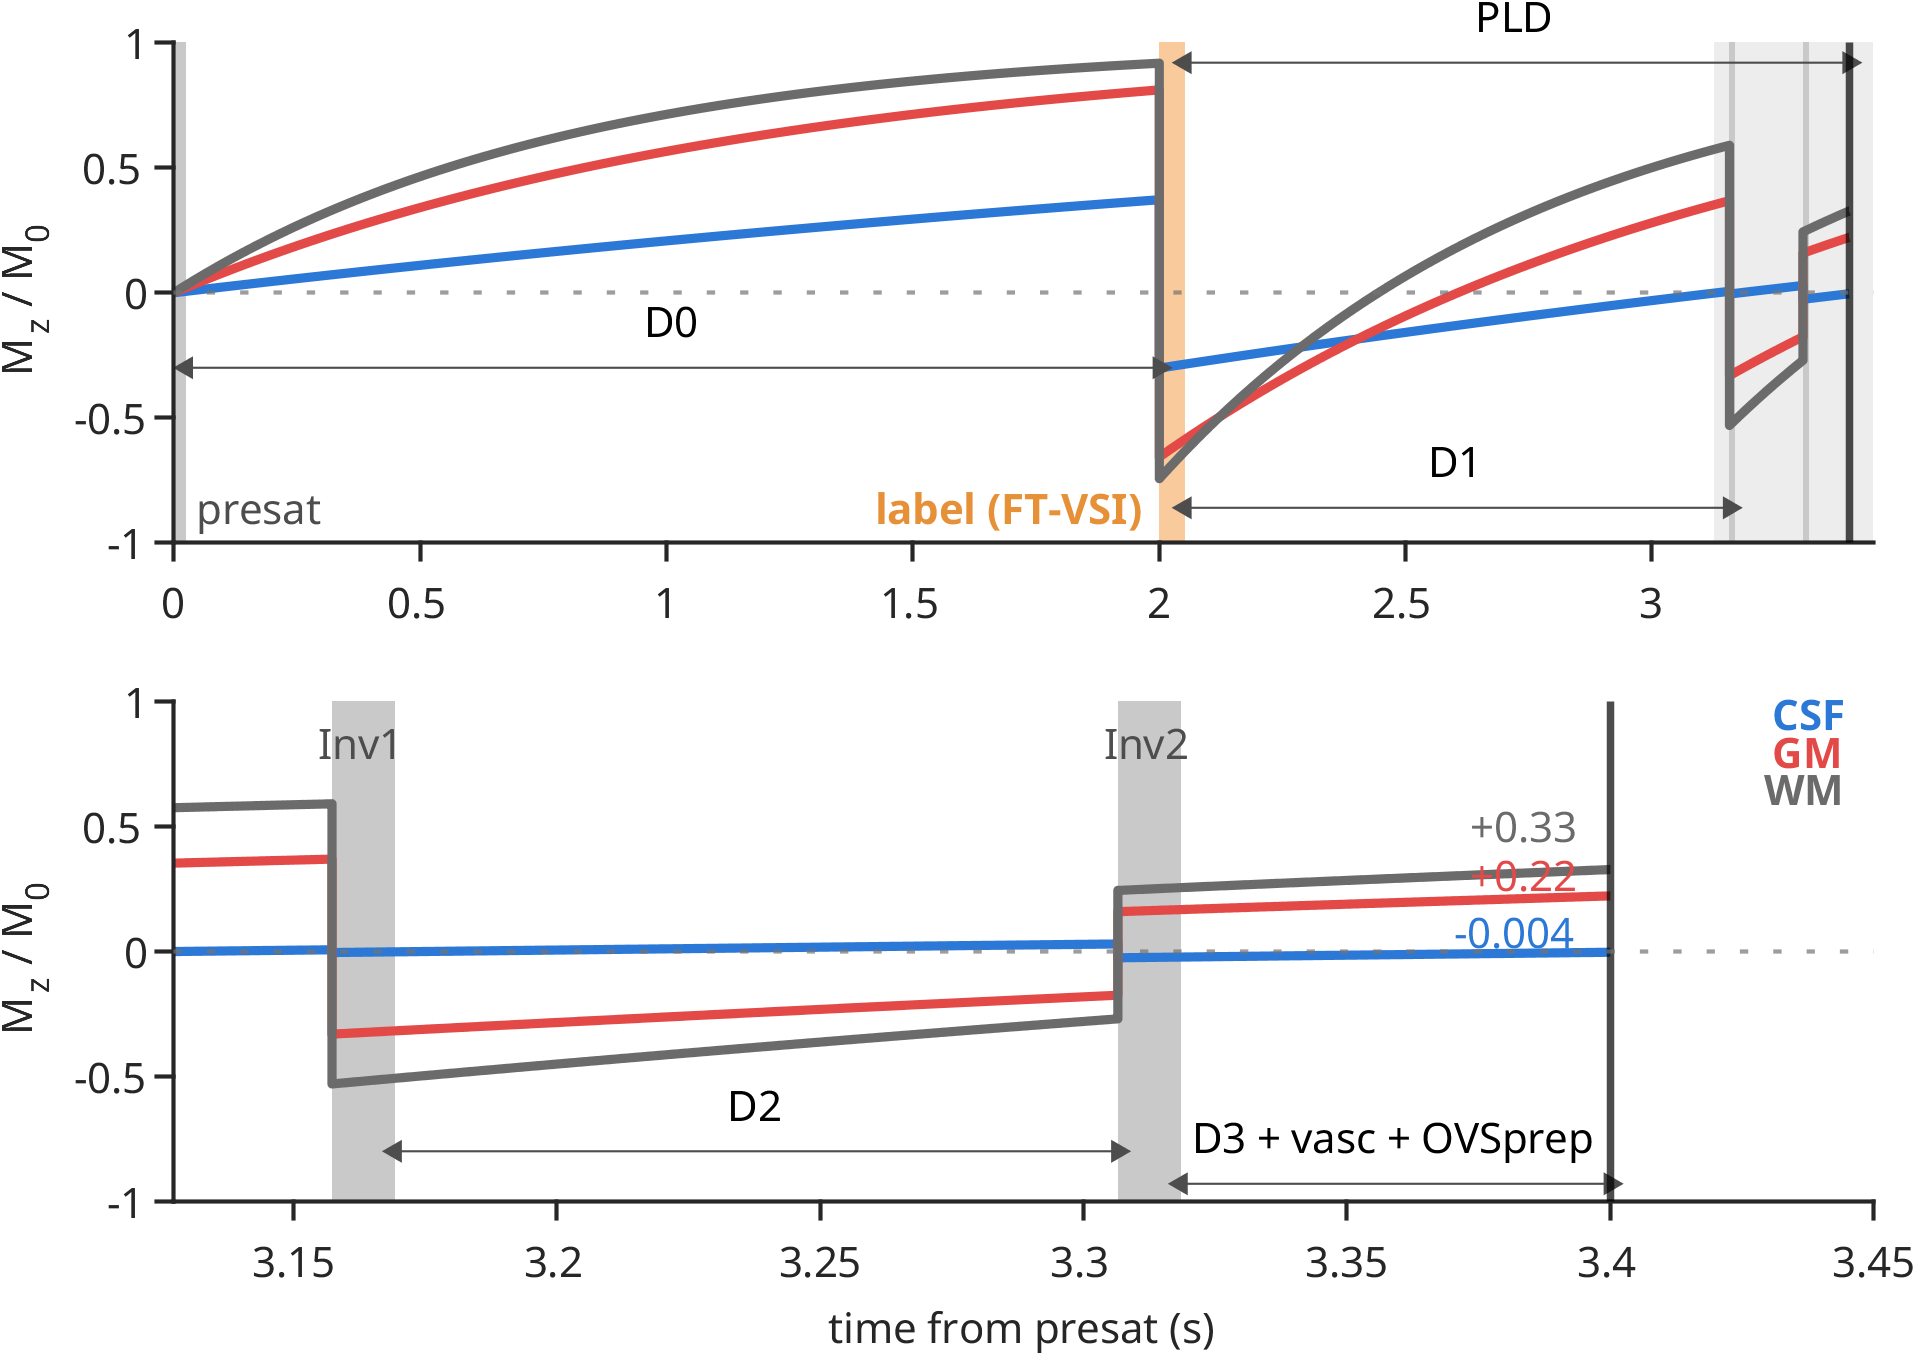
\includegraphics[width=17cm]{../figures/fig2_bgs_timing.png}};
  % normalized image coordinates: (0,0) bottom-left, (1,1) top-right
  \begin{scope}[x={(img.south east)}, y={(img.north west)}]
    % top of each panel's axes (1 - pixel row/1354): rows 45 and 703; letters sit in the
    % blank corner left of the y tick labels, above the M_z/M_0 label
    \node[anchor=north west, font=\bfseries, inner sep=0] at (0,1)     {(a)};
    \node[anchor=north west, font=\bfseries, inner sep=0] at (0,0.512) {(b)};
  \end{scope}
\end{tikzpicture}
\end{document}
